\usetikzlibrary{arrows.meta}
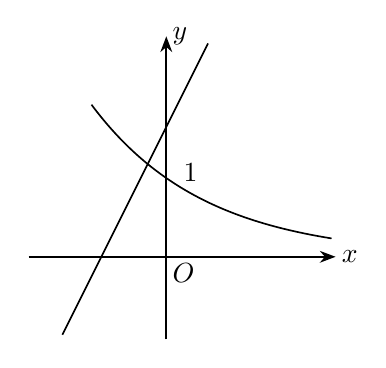
\begin{tikzpicture}[x=1cm,y=1cm,line width=.6pt,>=Stealth,font=\normalsize]
\coordinate (O) at (0,0);
\coordinate (Y1) at (0,1);
\coordinate (XA) at (-1.75,0);
\coordinate (XB) at (2.15,0);
\coordinate (YA) at (0,-1.05);
\coordinate (YB) at (0,2.8);
\coordinate (LS) at (-1.32,-0.99);
\coordinate (LE) at (0.53,2.71);
\draw[->] (XA)--(XB);
\draw[->] (YA)--(YB);
\draw (LS)--(LE);
\draw[domain=-0.95:2.1,samples=121] plot (\x,{pow(0.5,\x)});
\node[right=2pt,inner sep=0pt] at (XB) {$x$};
\node[right=2pt,inner sep=0pt] at (YB) {$y$};
\node[below right=2pt,inner sep=0pt] at (O) {$O$};
\node[right=6pt,yshift=2pt,inner sep=0pt] at (Y1) {$1$};
\end{tikzpicture}
